\documentclass[11pt,phd]{byuprop}
% Options for this class include the following (* indicates default):
%
%   10pt -- 10 point font size
%   11pt -- 11 point font size
%   12pt (*) -- 12 point font size
%
%   ms -- produce a thesis proposal (off)
%   areaexam -- produce a research area overview (off)
%   phd -- produce a dissertation proposal (off)
%
%   singlespacing -- single-spaced lines
%   doublespacing -- double-spaced lines
%
%   layout -- show layout lines on the pages, helps with overfull boxes (off)
%   grid -- show a half-inch grid on every page, helps with printing (off)


% This command fixes my particular printer, which starts 0.03 inches too low,
% shifting the whole page down by that amount.  This shifts the document
% content up so that it comes out right when printed.
%
% Discovering this sort of behavior is best done by specifying the ``grid''
% option in the class parameters above.  It prints a 1/2 inch grid on every
% page.  You can then use a ruler to determine exactly what the printer is
% doing.
%
% Uncomment to shift content up (accounting for printer problems)
%\setlength{\voffset}{-.03in}

% Here we set things up for invisible hyperlinks in the document.  This makes
% the electronic version clickable without changing the way that the document
% prints.  It's useful, but optional.  Note that if you use latex instead of
% pdflatex, you should change "pdftex" to "ps2pdf".
\usepackage[
    pdftex,
    bookmarks=true,
    breaklinks=true,
    raiselinks=true,
    pdfborder={0 0 0},
    colorlinks=false,
    ]{hyperref}
\usepackage{graphicx}
\usepackage{caption}
\usepackage{subcaption}

% Rewrite the itemize, description, and enumerate environments to have more
% reasonable spacing:
\newcommand{\ItemSep}{\itemsep 0pt}
\let\oldenum=\enumerate
\renewcommand{\enumerate}{\oldenum \ItemSep}
\let\olditem=\itemize
\renewcommand{\itemize}{\olditem \ItemSep}
\let\olddesc=\description
\renewcommand{\description}{\olddesc \ItemSep}

% Get a little less fussy about word spacing on a line.  Sometimes produces
% ugly results, so keep your eyes peeled.
\sloppy

% Important settings for the byuprop class. %
%%%%%%%%%%%%%%%%%%%%%%%%%%%%%%%%%%%%%%%%%%%%%

% Because I use these things in more than one place, I created new commands for
% them.  I did not use \providecommand because I absolutely want LaTeX to error
% out if these already exist.
\newcommand{\Title}{Computational Creativity in Popular Music Composition}
\newcommand{\Author}{Paul M. Bodily}
\newcommand{\SubmissionMonth}{December}
\newcommand{\SubmissionYear}{2015}

% Take these from the commands defined above
\title{\Title}
\author{\Author}
\monthsubmitted{\SubmissionMonth}
\yearsubmitted{\SubmissionYear}

% Committee members
\committeechair{Dan~Ventura}
\committeemembera{Neil~Thornock}
\committeememberb{Mark~Clement}
\committeememberc{Christophe~Giraud-Carrier}
\committeememberd{Seth~Holladay}

% Department graduate coordinator
\graduatecoordinator{Quinn~Snell}

\documentabstract{%
% The proposal abstract should be 1 to 2 paragraphs.
What is human creativity and how can we create machines that are creative? Significant progress has been made towards developing intelligent machines, but the most valued contributions to society go beyond intelligence. They require creativity---the ability to innovate novelty and value. Creativity and its fruits are highly valued in all societies. New concept-learning approaches to machine learning show an impressive ability to identify and generate new instances of an idea with only one or few examples. These new approaches are able to learn \emph{concepts}---much like we do---which can then be reused and combined to quickly understand and innovate related concepts. 

We hypothesize that concept-learning approaches are effective in developing creative machines. We propose to test this hypothesis in the context of developing a lyrical song generation model. We will use the paradigm of a graphical model which models independence assumptions between the various subtasks of composition in order to focus on each subtask individually. We intend to use a combination of data-driven and rule-based approaches. Inasmuch as creativity in humans is generally defined together with an inspiring idea or mood, we likewise incorporate such a module in our system. We will evaluate the model's ability to simulate human-like creativity using a combination of quantitative metrics and qualitative surveys.
}

%%%%%%%%%%%%%%%%%%%%%%%%%%%%%%%%%%%%%%%%%%%%%

% Set up the internal PDF information so that it becomes part of the document
% metadata.  The pdfinfo command will display this. Be sure to set the document
% type and add your own keywords.
\hypersetup{%
    pdftitle=\Title,%
    pdfauthor=\Author,%
    pdfsubject={Document Type, BYU CS Department: %
                Submitted \SubmissionMonth~\SubmissionYear, Created \today},%
    pdfkeywords={},%
}

% These packages allow the bibliography to be sorted alphabetically and allow references to more than one paper to be sorted and compressed (i.e. instead of [5,2,4,6] you get [2,4-6])
\usepackage[numbers,sort&compress]{natbib}
\usepackage{hypernat}

% Additional packages required for your specific thesis go here. I've left some I use as examples.
\usepackage{graphicx}
\usepackage{pdfsync}

\begin{document}

% Produce the preamble
\maketitle

%%%%%%%%%%%%%%%%%%%%%%%%%%%%%%%%%%%%%%%%%%%%%%%%%%%%%%%%%%%%%%%%%%%%%%%%%%%%%%%
\section{Introduction}
% 1-2 pages
% Answers:
% 1) What problem do you want to solve?
% 2) Who cares about this problem and why?

%What problem do you want to solve? What broader field of computer science does this relate to?

How are people so \emph{creative} and how can we develop machines that act \emph{creatively}? Rapid progress has been made towards achieving human-level performance in a variety of \emph{intelligence} tasks, for example, object recognition, language acquisition, and speech recognition. But \emph{creative} machines are yet in their infancy. Imagine a machine that crafts business strategies, develops military plans, engineers football plays, writes inspiring literature, or composes evocative music. Imagine a system whose knowledge and sensitivity combine to act in creative ways to respond to (and even improve) a user's state of being. What ideas could be generated? What value could be added to society?

Creativity is inherently difficult. It draws on the full gamut of intelligent abilities. It ventures into a realm where ``notions of optimality are \emph{not} defined''~\cite{eigenfeldt2012evaluating} (emphasis added). It defies norms, ignores risks, and breaks rules. It is unpredictable and serendipitous---seemingly at complete odds with the monotone consistency of a CPU. It necessitates not only the ability to generate solutions but also the capacity to be self-critical. This confluence of high pay-offs and high challenge has caused some to characterize computational creativity as ``a frontier for AI research beyond all others---maybe, even, the final frontier''~\cite{colton2012computational}. 

Recent research in Hierarchical Bayesian learning has achieved amazing progress in using human-like concept learning in order to perform one-shot classification, generation, and even new concept generation of handwritten characters, a traditional AI task \cite{Lake11122015}. This approach aims to learn concepts---much like we do---which are reused and combined to quickly understand new concepts in order to perform intelligence tasks. Can these same probabilistic models be applied to create machines that facilitate human-like \emph{creativity}? We propose to investigate this question in depth. We will concentrate our investigation on the specific computational creativity task of pop music generation as a concrete example of this endeavor. By forming our questions in this particular domain, we hope to find answers that can be applied generally to develop creative machines in other domains.

%Who cares about this problem and why?

Music and natural language are two characteristically human attributes. Of particular interest is the creative ability to write lyrical songs, a creative endeavor requiring both music \emph{and} natural language. Though each has an extensive history in AI (and CC), strangely their overlap is a relatively unexplored domain. As relates to using hierarchical concept learning, we stand to gain much from studying how we can combine two relatively well-studied disciplines to formulate a third. When properly synchronized, the affect of their combination is more than the sum of their parts.

There is widespread interest in automating the generation of creative, lyrical songs. Video game designers are increasingly investing in procedural content generation (including music) to better personalize the gaming experience~\cite{togelius2011search,lebaron2015intelligent}. Psychologists tout the effectiveness of using music to regulate mood and trigger strong emotional experiences~\cite{gabrielsson2001emotions}. YouTubers, who upload hundreds of hours of video every minute, face the challenge of finding (royalty-free) music to complement their new clips\footnote{e.g., see https://www.youtube.com/audiolibrary/music}. Artists invest enormous time and money into commissioning or composing original songs to meet the insatiable demand for another pop hit. A concept-based learning system that can generate personalized, sentiment-driven music would fuel a wave of possibility and innovation.

In addition, companies like Spotify, Apple, and Pandora gain enormous revenue from successfully recommending music attuned to a listener's preferences. This recommendation is limited A) by the system's ability to learn conceptually what drives a listener's tastes and B) by the availability of music that fits those tastes. A concept-based learning system that is capable of addressing both of those issues would be not only revolutionary, but also very profitable.

Lyrical song-writing poses a unique set of challenges. Linguistic challenges include: developing a cohesive lyrical text under the organizational constraints of (occasionally complex) rhyme schemes; text composition within verse/chorus structures that is both independently-meaningful and globally-coherent; and use of effective metaphors, dramatic tag lines, and other common lyrical elements. Musical challenges include: generation of melody to appropriately match and emphasize lyrical syllables; shaping of melody and harmonization to effect the mood expressed in the lyrics; the creation of singable melodies (both in terms of range and structure); and, as with lyrics, the synthesis of melody and harmony that is independently-meaningful and globally-coherent.

To be clear, our focus is on the generation of written, lyrical songs, with less regard to how these songs are acoustically performed. We have chosen to emphasize in pop music, insofar as pop music represents the genre that is currently most in demand.

Pop music is a genre with unique opportunities for CC research. Popular music is predominantly defined by lyrical compositions. Unlike generating lieds~\cite{toivanen2013automatical} or jazz leadsheets~\cite{pachet2014imitative}, pop songs generally have a unique hierarchical structure: multiple, connected verses that develop a common theme, interspersed with choruses or other segments. A wealth of data is available for pop music research in the form of online databases containing song-specific lyrics, harmony, structural organization, and metadata leveraged from crowd-sourcing efforts. Pop music is an emotionally charged genre---a characteristic which is heightened by the addition of lyrics---which provides an excellent medium through which to examine the generation of artifacts with \emph{musical meaning} (i.e., referencing an inspiring theme, mood, or intention). This referential or descriptive aspect of music is a ubiquitous element of human creativity~\cite{papadopoulos1999ai}.

A leadsheet for jazz music has been previously defined in~\cite{pachet2014imitative}. However, this previous definition requires adaptation in order to include lyrics. We therefore define a lyrical leadsheet as three ``parallel'' sequences: one that contains chord labels; a second that contains notes; and a third that contains lyrics. A \emph{chord label} is a triplet $<R, T, d>$, where $R$ is a pitch-class (e.g., C), $T$ is a chord type (e.g., `M7'), and $d$ is the duration. A \emph{note} is also a triplet $<p,d,s>$, where $p$ is the pitch (e.g., a MIDI-pitch between 0 and 127 or a rest), $d$ is the note duration, and $s$ is the lyrical syllable associated with the note. A lyricized leadsheet is a pair $<C, N>$ where $C = (C_1,...,C_k)$ is a temporal sequence of chord labels and $N = (N_1,...,N_l)$ is a temporal sequence of notes. $C$ and $N$ have the same total duration. We assume a one-to-one relationship between non-rest notes and syllables.

Our goal is to develop a system that addresses both musical and linguistic challenges to generate lyrical leadsheets in the genre of pop music, based on an inspiring theme or idea. In the interest of time, we expect to devote a greater portion of our energy to the musical challenges using mostly template-guided approaches to address the lyrical challenges.

%	"People find the difference between random arrangements of notes and the music of their native culture as obvious as the difference between random arrangements of words and meaningful sentences of their native language" (Mark Steedman, 1984)

%%%%%%%%%%%%%%%%%%%%%%%%%%%%%%%%%%%%%%%%%%%%%%%%%%%%%%%%%%%%%%%%%%%%%%%%%%%%%%%
\section{Related Work}

Much of the previous work done in AI with relation to music and language composition comes to bear on solutions to the lyrical song-writing task. Following a brief review of previous work in these more general subfields of AI, we look at what others have attempted with respect to the problem of lyrical song-writing. The remainder of the document will then detail the implementation (and validation) of a novel computationally-creative lyrical song-writing system.

%%%%%%%%%%%%%%%%%%%%%%%%%%%%%%%%%%%%%%%%%%%%%%%%%%%%%%%%%%%%%%%%%%%%%%%%%%%%%%%
\subsection{Research Area Overview}
% Research Area Overview
% Describes the broad research area (citing the 20 most important papers)
% Should be about 3 pages and may be in the Introduction or Related Work
% sections or may be an appendix.
%
%The field of computational creativity in music is couched within the broader context of Artificial Intelligence (AI). Much of the tools and techniques that have been used in AI research---especially in AI work related to music---carries over to lay the groundwork for .
%
%Assuming for the moment that computationally creative systems do exist, we might reasonably ask ``at what point does a system become creative? For example, if a system generates only a melody, but no harmony, can it be considered creative?'' Defining the boundary of creativity is difficult and certainly beyond our scope. However, any system which pretends to combine multiple elements of composition into a single artifact would benefit immensely from a consideration of what broader research has been done in considering each of the pieces separately, regardless of what ambitions that research had towards creating a creative system.
%
%A great number of diverse computational questions have been posed related to music. Those related to notes. Those related to harmonic progression. Those related to phrase expressions. Those related to classification, those related to prediction, and those related to generation.
%
%Music representations: Pachet (2014, jazz leadsheet generation) and Conklin and Witten (1995, MVP Systems)
%
%Despite the variety of questions, several specific computational methods have been repeatedly used to address them: (devote Overview to these, highlighting their relevance to what I'm about to do).
%
%Markov models: Ames (1989, markov in review), Papadopouos (2014, plagiarism), Meyer (1957, meaning and Info theory)
%
%Grammars: Steedman (1984, jazz grammar), Steedman (2014, parser for chord seqs)
%
%Evolutionary methods (Bown?)
%
%Knowledge-based systems
%
%ML and ANN
%
%These are the authors that are good in this area: Conklin and Witten*, Steedman*, Cope, Wiggins*, Papadopoulos*, Meyer, Pachet*, Ebcioglu, Widmer, Ames, Bown

%Within AI and machine learning, what sets of problems do you deal with? Is there work here that you plan to leverage?

For decades AI researchers have been interested in the problem of algorithmic composition in various forms. The breadth of problems that have been addressed ranges from composing melodies, to harmonizing existing melodies, to live jazz improvisation. Despite this breadth, the range of solutions is somewhat narrower. These approaches represent a valuable toolset in considering the generation of lyrical pop song generation. They include knowledge-based systems, grammar-based systems, Markovian systems, evolutionary systems, and machine learning systems (\cite{papadopoulos1999ai} provides a more complete survey).

%Meyer 1957 meaning in music and information theory.

David Cope in the 80's and 90's developed a system entitled Experiments in Musical Intelligence (EMI) with the goal of generating new compositions in the styles of various composers~\cite{cope1996experiments}. EMI's widely-acclaimed success is rooted in the extraction and recombination of patterns in the works of a selected composer. This approach is representative of knowledge-based systems, which employ explicit reasoning via sets of rules or constraints. The learning of stylistic patterns might also be considered a generative grammar approach to composition, where the grammar is induced from an artist's collective works. Cope's EMI was largely constructed to emulate classical and ragtime composers, where the domain is devoid of lyrical melodies. 

Mark Steedman is known for using manually crafted grammars for generating twelve-bar jazz chord sequences. His 1984 paper demonstrates how the variety of chord progressions manifest in twelve-bar jazz tunes can all be explained using a set of hand-crafted rules~\cite{steedman1984generative}. Johnson-Laird also employ a grammar for the generation of jazz chord sequences~\cite{johnson1991jazz}. 

Markov models represent another common approach to algorithmic composition. Ames demonstrates the computation of transition matrices of varying orders in order to predict what comes next in a sequence of states given the preceding context~\cite{ames1989markov}. States may be notes, chords, or even phrase expressions.

As an augmentation to the Markov approach, Conklin and Witten describe multiple viewpoint systems, which allow several facets (e.g., duration, pitch, volume) of a musical expression to be encoded as a single token, rather than modeling each aspect of the music with a different model~\cite{conklin1995multiple}.

CHORALE is another commonly cited knowledge-based system~\cite{ebciouglu1988expert}. Designed to harmonize Bach chorales, this system employs multiple viewpoints in its layout of 270 (fairly complex) rules. As is common with rule-based systems, an exhaustive set of rules is generally unachievable. Numerous exceptions remain unaccomodated.

Ramalho and Ganascia aim at simulating creativity via intention-based real-time jazz improvisation~\cite{ramalho1994simulating}. They leverage Pachet's notion of potential actions (PACTs) to describe intention in music~\cite{pachet1991representing}. A PACT represents a procedural (e.g., play a particular rhythm, play an ascending arpeggio) or property-setting (e.g., play loud, use the major scale) characteristic of music which serves to guide the composition according to specific intentions. This intention-based approach is supported by previous research which experimentally demonstrates the important role of contour in how tonal music is perceived ~\cite{dowling1978scale}.

%ML and ANN
%Evolutionary

%%%%%%%%%%%%%%%%%%%%%%%%%%%%%%%%%%%%%%%%%%%%%%%%%%%%%%%%%%%%%%%%%%%%%%%%%%%%%%%
\subsection{Research-Related Work}
% Related Work
% 1-2 pages
% Answers:
% 3) What have others done to solve this problem and why is this inadequate?
%    (only a small overlap with the area exam from the introduction)
%The specific question I'm interested in is Can a computer be programmed to generate artifacts in the genre of popular music that, if generated by a human, would be deemed creative? These methods I've outlined above have been employed by the following studies to try and solve this problem (or closely related problems) with the following results. In all cases, they fall short of what I hope to accomplish either because they have not examined pop music (with its structure and lyrical components), they were not attempting to implement a \emph{creative} system, or they were not attempting to compose an entire piece.

%What is the particular problem that your dissertation topic is concerned with? What has been done by others to solve this problem and why is it inadequate?

The problem of generating lyrical songs is relatively new and unexplored, particularly in the pop music genre. We examine a few of the closest related projects here.

Pachet and Roy introduce the problem of generating musical leadsheets in the style of a particular composer~\cite{pachet2014imitative}. They formally define a leadsheet as a parallel sequence of chords and notes. In the jazz domain, this would be considered a full composition. Musical generation is accomplished with composer-specific training of Markov models. Their results indicate that leadsheets generated in the style of a specific composer are correctly classified with accuracy comparable to classification of original leadsheets heldout from the training dataset. Though sufficient for jazz compositions, the additional complexity of pop music lyrics and verse/chorus structure generation remains unaddressed by this approach. 

Toivanen et al. describe M.U. Sicus, a system which generates novel lieds (art songs) in a particular mood with lyrics composed in the Finnish language~\cite{toivanen2013automatical}. Building on previous research into the generation of poetry, M.U. Sicus generates (in order) lyrics, rhythm, chords, and then melodies using a combination of grammar-induction and Markovian approaches. We plan to approach the problem in a similar manner, but with the added complexity of integrating verse/chorus structure. We plan to more carefully evaluate the alignment of strong versus weak syllables and the melody, which M.U. Sicus does not consider.

Monteith et al. generate melodic accompaniment for existing lyrics in order to generate new lyrical compositions~\cite{monteith2012automatic}. They also create a data-driven dictionary from which rhythms are selected and melodies are generated according to a trained $n$-gram model. They generate melodies in three different genres for lyrics sampled from the same three genres and find that in many cases, the computer-generated melodies are found to fit better and be more pleasing than the original melodies as evaluated by a panel of human judges. The tasks of generating lyrics and generating harmony are not addressed.

Scirea et al. recently published the Scientific Music Generator (SMUG), which generates lyrics (inspired from academic papers) and accompanying melodies~\cite{scirea2015smug}. They sample lyrical substructures from a small database of existing pop songs which they use to construct new lyrical compositions. They use Markov models, modified via genetic algorithms, to generate sequences of notes and rhythms. Although they have a complete pipeline that generates lyrical compositions, the lyrical model lacks sufficient complexity to generate grammatical or semantic coherence.

Chuan and Chew generate and evaluate musical harmonizations that emulate style in popular music~\cite{chuan2011generating}. They generate the chords from the melody, using Markov chains to model the likelihood of chord patterns. Melody fragments that strongly imply certain chords are used as anchors which are connected using chord sequences generated by consulting the Markov chains. They focus on Western popular songs. They don't address lyrics, nor do they generate melodies.

None of the existing systems explore structure, structure-specific models of harmony, or investigate the plausibility of using a hierarchical model to incorporate these elements with elements of harmony, melody, and lyrics to effect human-like creativity. Our purpose is to develop such a model, as we describe in the sections below.

%%%%%%%%%%%%%%%%%%%%%%%%%%%%%%%%%%%%%%%%%%%%%%%%%%%%%%%%%%%%%%%%%%%%%%%%%%%%%%%
\section{Thesis Statement}
% 1 to 2 sentences
%A probabilistic graphical model which learns data-driven distributions for individual components of structure, chords, melody, and lyrics is able to generate novel popular music leadsheets which demonstrate human-like creativity in terms of novelty, surprise, and value.

A probabilistic model which uses a combination of data-driven solutions and rule-based solutions for individual distributions of structure, chords, melody, and lyrics is able to generate novel lyrical leadsheets in the western popular music genre which demonstrate human-like creativity in terms of novelty, surprise, and value.

%%%%%%%%%%%%%%%%%%%%%%%%%%%%%%%%%%%%%%%%%%%%%%%%%%%%%%%%%%%%%%%%%%%%%%%%%%%%%%%
\section{Project Description}
% about 6-8 pages
% Answers:
% 4) What is your proposed solution to this problem?

%An algorithmic composition in the popular music genre involves generating several components: shape (global, local), chord progression (root, chords, durations), chord voicings, melody (rhythm, pitch, duration), and lyrics (syllabic decomposition, rhyming). We can represent each of these components as a discrete random variable  ($S$, $C$, $V$, $M$, and $L$ respectively).  Furthermore, we presume that musical creativity (as expressed by humans) is almost always motivated by an emotion or other inspiration source, $I$. The problem of probabilistically generating an algorithmic composition might be formally defined in terms of the joint probability distribution of these six variables:
%
%\begin{center}
%$P(S, C, V, M, L, I)$
%\end{center}
%
%Composers are commonly asked, ''What do you compose first? Melody, chords, or lyrics?" Each composer will respond differently. It is not uncommon for a composer to use different approaches with different compositions. Some composers respond that two or three of these elements are simultaneously created first. Despite this variety in response, most composers will generally express a preference for the order in which they create music.
%
%This preferential ordering of the composed elements suggests that the problem of pop music generation might be simplified by factoring the joint distribution according to a set of formal independence assumptions between the compositional components. The set of assumptions that may be adopted will vary just as a composers preferred order. We propose one such set of assumptions which we will use throughout our experiments (see Fig.~\ref{fig:graphical_model}):
%
%\begin{figure}
%  \centering
%  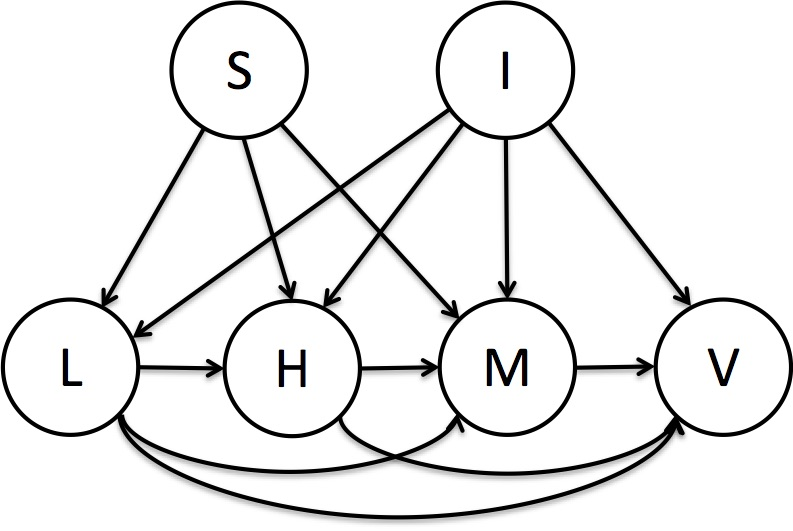
\includegraphics[width=.35\textwidth]{graphics/graphical_model.jpg}
%  \caption{A probabilistic graphical model for pop music generation based on a set of independence assumptions. The assumptions shown might be comparative to a composer who strictly prefers to generate music in order of chord progression, melody, and then lyrics.}
%    \label{fig:graphical_model}
%\end{figure}
%
%\begin{itemize}
%\item{$C$ depends on $S$ and $I$}
%\item{$M$ depends on $C$, $S$, and $I$}
%\item{$L$ depends on $M$, $S$ and $I$}
%\item{$V$ depends on $C$ and $I$}
%\item{$S$ and $I$ are unconditionally independent}
%\end{itemize}
%
%We can thus factor our joint probability according to these independence assumptions as:
%
%\begin{center}
%$P(S, C, V, M, L, I) = P(C | I, S) P(M | C, S, I) P(L | M, S, I) P(V | C, I) P(S) P(I)$
%\end{center}
%
%The beauty of this factorization is that we can now focus separately on how to represent the distribution for each factor. This modular framework also allows comparison of multiple solutions for each component. We will examine each of these factors individually. For each distribution we will describe 1) a simple, dummy solution in order to provide baseline functionality to the overall framework and 2) one or more novel creative solutions. 
%
%\subsection{$P(S)$}
%
%Can we learn a grammar that would allow us to generate structures, clear to chord symbols? Would this grammar capture ideas like verses and choruses?
%
%Can we simply learn more distributions for each level of structural hierarchy? E.g., can we create a distribution over verse-chorus-bridge segmentation schemes and then another distribution for the segmentation schemes of each of those elements?
%
%Unlike formulaic structures like 12-bar blues (Steedman, 1984), many pop songs can have widely varying structures.
%
%Lots been studied on structure, see Steedman, 2014, intro paragraph.
%
%Suffix Arrays to find patterns
%
%Matrix to find patterns
%
%High-level structure vs low-level structure
%
%\subsection{$P(C | I, S)$}
%
%We want to learn from data ``idiomatic chord progressions'' (see Keller, Winter 2013, CMJ) , but also to go a step farther in finding ways to combine these idioms to form novel chord progressions, similar, perhaps to a crossover procedure in a genetic algorithm. 
%
%"progressions as bigger thoughts than just chords or pairs of chords in isolation. It is helpful for the player to recognize and appreciate certain idiomatic chord progressions, as many progressions recur across the space of tunes" (Keller, 2014)
%
%It's okay to ignore suffixes for chords and focus on the base chord. "Those that appear in brackets are relatively unimportant
%and will be ignored until the section on the grammar" (Steedman, 1984).
%
%I realized something important today: generally, even if chords are wrong in a database, they were nonetheless deemed right by some human somewhere and generally represent acceptable progressions, even if not those from the original composer. In other words, chord charts could from one perspective be viewed as compositions of those who transcribed them, which is still something worth learning from a computational perspective.
%
%The dumb answer is simply to use something like HookTheory to get transition probabilities. We can generate forwards and/or backwards (and should compare both). The chords will depend on the high-level structure and the lower level structure. 
%
%Avoiding plagiarism?
%
%\subsection{$P(M | C, S, I)$}
%
%"There are some musical questions about systems which only generate melodies (e.g., Todd, 1989; Ralley, 1995; Spector and Alpern, 1995). How can we expect to evaluate the musical output if we do not have a harmonic context for it? Most melodies will sound acceptable in some context or other." (Papadopoulos and Wiggins, 1999).
%
%The melody at any given point depends on what came before it, whether it is a downbeat, the current chord, the structure (e.g., segments repeat melodies), possibly the contour of the line. Note durations depend on the inspiring idea. Note pitches depend indirectly on the inspiring idea via the chord progression. 
%
%Avoiding plagiarism.
%
%Use mathematical regression (of note frequencies?) to look at contours of notes?
%
%DNA-inspired?
%
%\subsection{$P(L | M, S, I)$}
%
%Once we have a melody, we must then find words to fit the melody. It is possible that lyrics may come before melody. The lyrics depend heavily on the inspiring idea. We need to choose the point of view (e.g., first person, second person, third person, etc). Given then a point of view and an inspiring idea, we must come up with phrases of a particular length (in syllables) or which combine to form phrase blocks of a particular length. We must incorporate into our model the ability to rhyme in accordance with the meter and rhyme scheme. We would also like to have some semantic web which allows us to use metaphors, similes, personification, alliteration. We want to find words that are more heavily charged, perhaps as determined by looking at exclamation points on Twitter or something. Of course, we need explicit language filters.
%
%See http://www.datamuse.com/api/ for a great database that encompasses thesaurus, specific ending or starting letters, rhymes, or specific word lengths, or words spelled similar to other words, maybe even part of speech.
%
%See http://www.programmableweb.com/api/rhyming for an API to scrape and use Rhymezone.
%See http://rhymebrain.com/api.html
%Rhymezone is easily scraped and has lots of real prose examples.
%
%Look at dictionaries for word type, syllable count, pronunciation, etc.
%
%Could learn n-gram model from other songs.
%
%How about using omdb to get proper nouns for similes or something (moves like Jagger)
%
%Avoiding plagiarism.
%
%\subsection{$P(I)$}
%
%We will initially randomly select one of 6 possible inspiring emotions: Love, Joy, Surprise, Anger, Sadness, Fear. In the future we may possible consider a more complex model that selects one of these emotions based on interaction with environmental circumstances (e.g., via sentiment analysis of newspapers, sporting event outcomes, stock market, weather, social network posts (pick an individual and mirror their emotions), etc).  Consider also the six Ekman emotions (Ekman, 1993; see their use by e.g., mihalcea, 2012)
%
%\subsection{$P(V | C, I)$}
%
%"The particular key used to accompany a melody is largely a matter of convenience, but the appropriate sequence of tonic, subdominant, and dominant chords is a fixed aspect of its meaning." (Steedman, 1984). In our model, key is determined by the range of notes in the melody (in order to be singable), with a preference towards simpler key signatures (i.e., fewer sharps or flats) or perhaps a preference for flats or sharps dependent on the mood. Time signature is likewise dependent on mood. Tempo, also.
%
%"The performance of a piece is another important factor and should not be regarded as irrelevant in the context of algorithmic composition." (Papadopoulos and Wiggins, 1999)
%
%Paper: Chord progression and plagiarizing. Could we conceive of chord progressions that are not already seen?! That would be quite creative, I think. It would represent an example of T-transformation, a new way of finding good solutions within the current domain. 
%
%Paper: Novel chord progression generation using Euclidean distance between chord substitution? 
%
%Paper: PCKY? 
%
%Paper: Emotion-inspired LEGO brick selection for generation of chord progressions.
%
%Paper: Examination of LEGO bricks in classical and pop genres. (See Keller winter, 2013 CMJ for details)
%
%Paper: Comparison of chord progression models between jazz, classical, and pop music
%
%Paper: Use simplicity of mathematical relationships between pitches to describe how good something sounds... consider tension.
%
%Paper: If you change the chord progression on the chorus, do people still recognize it as the chorus? If you change the lyrics on the chorus, do people still recognize it as the chorus?

Popular musicians are routinely questioned about their song-writing process. What comes first: The music? The lyrics? The chords? Answers vary sufficiently to suggest that there are numerous, equally successful approaches to the creation of new lyrical compositions. Though in some cases artists will insist that various elements are simultaneously generated, it is often the case that individual elements are composed under independence assumptions. For example, given a particular theme, an artist may entirely compose the lyrics before even attempting to compose the melody, or vice versa. 

Figure~\ref{fig:graphical_model} shows a graphical model that models a set of independence assumptions between the several subtasks of automated lyrical music generation in the genre of popular music. The set of independence assumptions will vary from one creative agent to another, and often a single creative agent may use a different creative model for different compositions. This particular set of independence assumptions represents the creative process that we intend to follow in this study. To model the lyrical leadsheet generation task in this way substantially simplifies the song-writing process insofar as solutions can be developed and evaluated modularly.

\begin{figure}
  \centering
  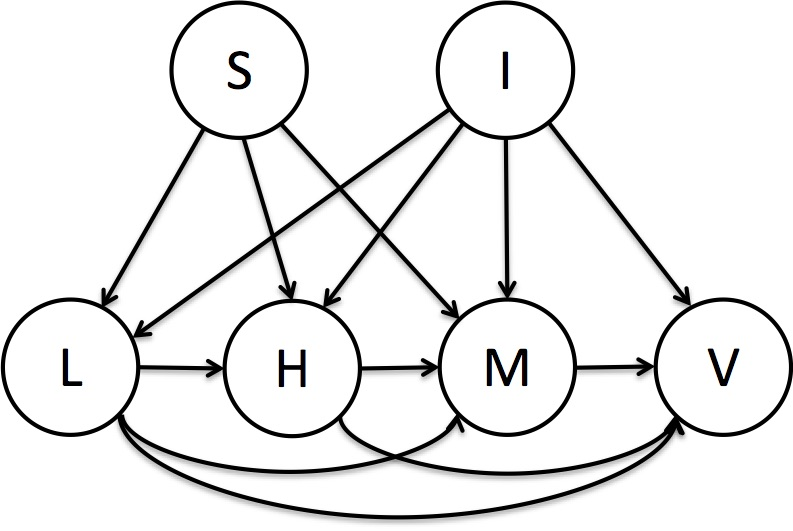
\includegraphics[width=.35\textwidth]{graphics/graphical_model.jpg}
  \caption{A probabilistic graphical model for pop music generation based on a set of independence assumptions. The model shown is comparable to a composer who strictly prefers to generate music in order of lyrics, chords, and then melody.}
    \label{fig:graphical_model}
\end{figure}

In plain English, the model essentially outlines how a particular song-writer would go about composing a novel pop song. First, a global song structure $S$ (e.g., the sequence of verses, choruses, etc.) and a theme or inspiring emotion $I$ are determined. Given these two elements, the system then generates (in order) the lyrics $L$, the harmony $H$, the melody $M$, and the voicing $V$. A lyrical leadsheet $<C,N>$ is created by combining $L$ and $M$ to form $N$ and letting $C = H$. $M$ is generated under the constraint that it contains as many notes as $L$ has syllables. $S$ and $I$ have only an indirect influence on the definition of the lyrical leadsheet. $V$ refers to how the defined leadsheet is subsequently performed.

We plan to allow arbitrary selection of time signature between 3/4 and 4/4, as most popular music is written with these signatures. We will also assume that key signature remains constant for a given composition and is chosen as a function of the melody in order to make the song singable for a male tenor voice. In the following sections we define each of these elements in detail and discuss possible methods of implementation.  We propose to encode a fitness function for each module which is tuned to promote artifacts which best reflect attributes of creativity. Each module will thus be designed to both \emph{generate} and \emph{evaluate} artifacts in order to select a single choice for the compositional element.

In each case we propose a baseline (uncreative) solution and two possible creative solutions to each module. Except in the case of the lyrics module, we initially plan to only implement \emph{one} of the creative solutions. In the case of the lyrics module, for the sake of time we will focus on simply completing the baseline model. Should time allow (or if the first becomes for any reason infeasible), we will then consider the others. The dissertation will demonstrate that the combination of these solutions is sufficient to generating artifacts in the genre of popular music that pass the Turing test for computer creativity.

\subsection{Structure}

Repetition (e.g., of harmony, melody, or lyrics) is a critical component of successful pop music because it increases the ease with which information is processed by the brain~\cite{nunes2015power}.  We will refer to these patterns of repetition as the \emph{structure} of the composition. Though not required to define a lyrical leadsheet, modeling structure---both at a global and substructural level---is an essential characteristic of successful song-writing. 

\subsubsection{Global Structure}

The organization of a pop song into a sequence of segments\footnote{As a working definition, a \emph{segment} will refer to a unique (possibly repeated) subsequence of the composition. Thus a song with several verses will have a single ``verse'' segment. It should be noted that segment boundaries are not well-defined, and thus we might expect variability of segment labels by labeler. The exact labeling and assignment of segments is not essential to their effective use in recognizing a global structure of repetition.} (e.g., intros, verses, pre-choruses, choruses, bridges, outros, etc.) is a unique element of pop music. To our knowledge this \emph{global structure} (or \emph{structure}), though studied extensively with respect to the segmentation of audio signal~\cite{foote2000automatic}, has not been previously studied in the context of algorithmic composition. There is significant variety in the inclusion and ordering of the different segments (e.g., Figure~\ref{fig:segment_variety}) which adds to the novelty, surprise, and value of the composition. Consider, for example, the surprise/value of following a pre-chorus with something other than a chorus, as in Billy Joel's ``Piano Man''.

\begin{figure}
  \centering
  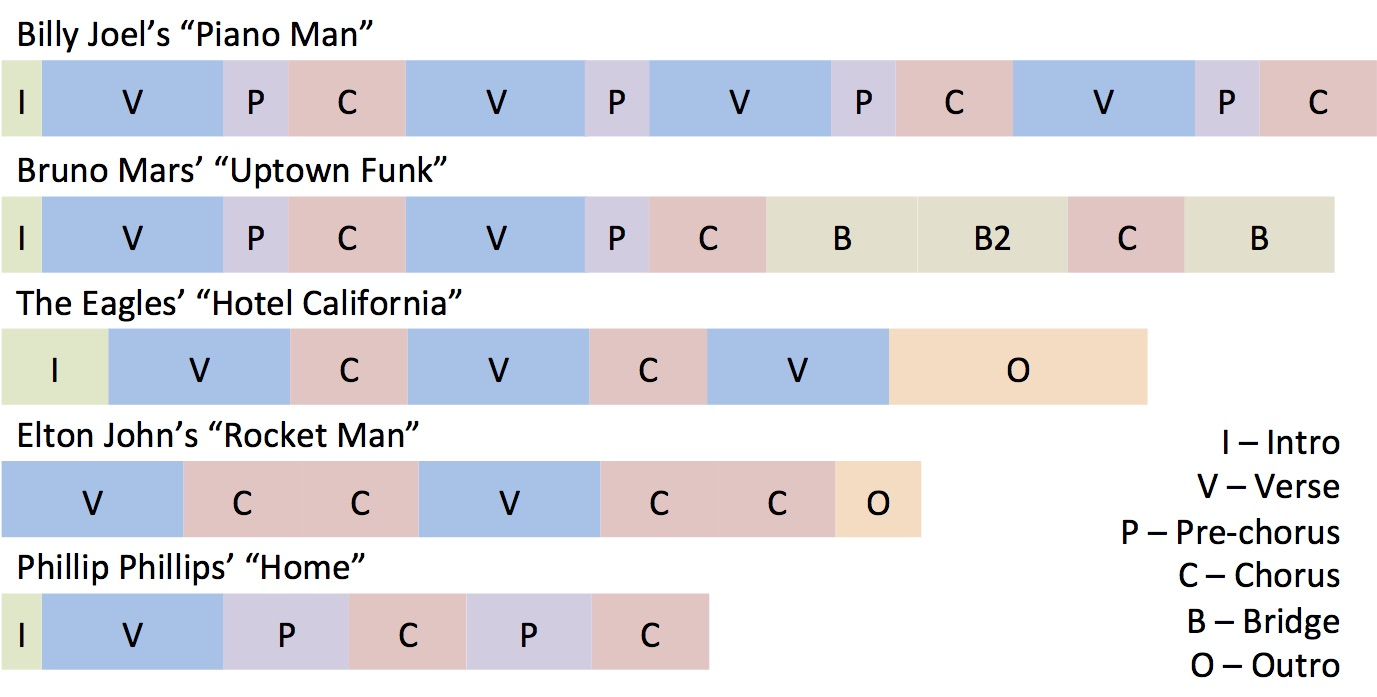
\includegraphics[width=.65\textwidth]{graphics/segment_variety.jpg}
  \caption{The inclusion and ordering of different song segments varies significantly, suggesting that global structure is a non-trivial creative aspect in the song-writing process.}
    \label{fig:segment_variety}
\end{figure}

A baseline solution to generating global structure is to always use the same static structure (e.g., intro, verse, chorus, verse, chorus, bridge, chorus). This would be selected according to the structure that is most common in our training data.

One creative solution is to learn a distribution of possible structures from data. The idea of elucidating patterns from a corpus has been applied to generate rhythms~\cite{monteith2012automatic} and lyrical substructures~\cite{scirea2015smug} but not at the level of global song structure. 

A second creative solution is to learn a structure grammar from data where segments compose the set of terminals. This, too, has been tried with respect to other elements of composition (e.g.,~\cite{steedman1984generative}) but not with global song structure. Compared to simply learning a distribution, a grammar has the added ability (for good or for bad) of creating structures that were not seen in the training set.

\subsubsection{Substructure}

There is really no limit to the degree of hierarchical repetition within a song (nor does it necessarily need to be strictly hierarchical). For example, consider Figure~\ref{fig:substructure_example}. ``Piano Man'' has four verses, each of which use the same harmonic progression, melody, and high-level rhyme scheme. Within this repeated verse segment, however, is layered additional repetition. The harmonic progression pictured in Figure~\ref{fig:substructure_example} represents a substructure whose progression and rhyme scheme is repeated twice for each verse and once in each chorus. Furthermore the pictured progression itself repeats the sub-substructure of C---G/B---F/A---C/G (which is also present in the introduction). A third substructure example is present in the lyrics. Whereas each repetition of this substructure rhymes words at the ends of the 2nd and 4th lines (e.g., ``smile'' and ``while''), five of the eight repetitions insert an additional substructural rhyme scheme in the 3rd line (e.g., ``me'' and ``see''). Learning patterns of repetition at several layers (and not just at the highest or lowest level) enables a generative system to create novel combinations of layered repetition for novel compositions.

\begin{figure}
  \centering
  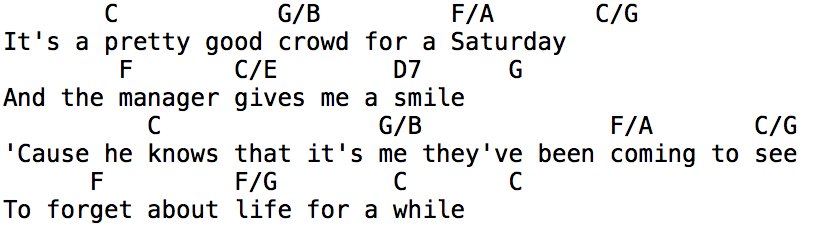
\includegraphics[width=.5\textwidth]{graphics/subtructure_example.png}
  \caption{Several layers of structural repetition beyond the repetition of verse and chorus structure contribute to effective compositions. These lines from the first verse of ``Piano Man'' represent a substructure that is repeated twice in each verse and once in each chorus. Additional layers of substructure exist even \emph{within} this substructure, demonstrating the effective use of hierarchical structure in pop music.}
    \label{fig:substructure_example}
\end{figure}

A baseline solution to generating substructure is to ignore it altogether. This would essentially result in songs where the only repeated elements are the segments themselves.

Any other solution will require the introduction of a substructural language capable of representing repetition of harmonic sequence and rhythm, melodic sequence and rhythm, lyrical phrases, and rhymed syllables. Though not all of these repeatable attributes are part of every repeated element, it is possible that some or all of them could be present together (e.g., in a chorus). %The development of a substructural language is a high priority in the next stages of our research.

With the aid of the substructural language, we can begin to consider other ways of generating substructures. One creative solution is to generate abstract, parameterizable substructures for song segments, each of which is itself composed of other abstract, parameterizable substructures (cf.~\cite{lebaron2015intelligent}) . The parameters might include one or more abstract patterns of repetition, the repeatable attributes to which they apply, the number of times the pattern repeats within the substructure, and the depth of the hierarchy of abstract substructures within the given substructure.

A second creative solution is to learn a substructure distribution from data. To increase the power of our data, we would learn a distribution for each repeatable attribute in order to then generate new combinations of repeatable attributes for substructure elements.

%\subsubsection{Local Variation}
%
%Though pop music commonly exhibits a global structure and several substructures, the ability to vary structure at each repetition of a segment is a critical element of creativity that introduces novelty and surprise. Such localized variation can be generated through specific rule-based algorithms during later generative modules or as a post-generative step. We plan to consider this only after we have found meaningful solutions to the rest of the generative process.

\subsection{Inspiring Idea}

A critical element of creativity is the theme (e.g., loneliness, courage, despair), mood (e.g.,  joy, anger, sadness), or intent (e.g., to inspire, to intimidate) that motivates the generation of new artifacts. As shown in the model, this inspiring idea is assumed to be derived independent of solutions to the other song-writing subtasks. The basis for this assumption is that a song-writer is not likely to select his/her intent or mood based on the song that he/she is composing, but rather vice versa. The lyrics, harmony, melody, and voicing are all carefully crafted to reflect this motivating thought. Often, the value ascribed to a human-generated artifact is determined by the success of these secondary components in transmitting the inspiring idea.

For our purposes, we limit inspiring ideas to emotions, with each composition being limited to a single emotion. At least two basic sets of emotions have been used in the CC literature~\cite{monteith2010automatic,mihalcea2012lyrics}. The first, outlined by Parrott~\cite{parrott2001emotions}, includes love, joy, surprise, anger, sadness, and fear. The second, outlined by Ekman~\cite{ekman1993facial}, includes anger, disgust, fear, happiness, sadness, and surprise. We propose to use the latter insofar as distinguishing in pop music between love and emotions such as joy or sadness is challenging.

A baseline solution to generating an inspiring idea is to select randomly or according to some distribution (learned via sentiment analysis of other lyrical and musical inspirations) from the set of possible inspiring ideas. 

One creative solution is to prompt the user for an inspiring idea from which to generate a lyrical composition. The system might then choose to either adopt the inspiring idea of the user, or alternatively to react to the user's emotion (e.g., a song to cheer up a sad user). 

A second creative solution is to select an inspiring idea based on interaction with an environment (e.g., via sentiment analysis of newspapers, sporting event outcomes, stock market, weather, social network posts, etc.). In this sense, our system would develop a \emph{persona}, whose interests and affiliations imitate those of a human, change over time, and continually provide varied inspirations for its generative process (see Figure~\ref{fig:inspiring_idea}).

\begin{figure}
  \centering
  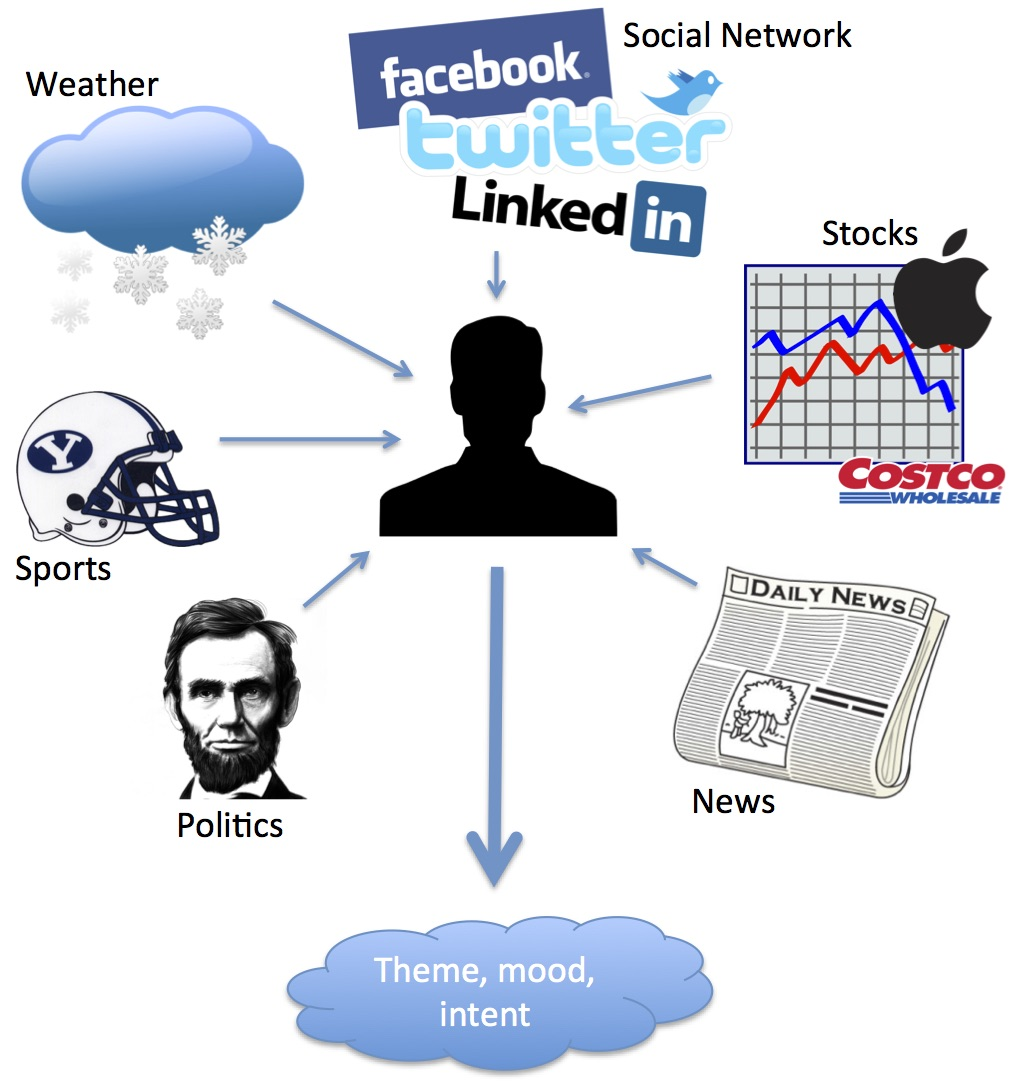
\includegraphics[width=.45\textwidth]{graphics/inspiring_idea.jpg}
  \caption{Creative artifacts are influenced by an inspiring idea that is affected by an agent's environment, interests, and affiliations.}
    \label{fig:inspiring_idea}
\end{figure}

\subsection{Lyrics}

The generation of lyrics requires more than generating simply meaningful, grammatical text; lyrics must also be poetic (both structurally and linguistically) and must effectively communicate the inspiring idea. Regardless of the melody to be generated, the lyrics comprise the most fundamental component in estimating a song's mood~\cite{chi2009power}.

In composing a pop song (where the length is commonly between one hundred and three hundred words), generating semantically coherent lyrics is quite challenging, requiring consideration of lexical choice, syntax, and semantics. Numerous approaches to this problem have been and might be proposed. Though well within the scope of our interest, time will likely limit how much we will be able to devote to this task. Thus, we propose here a few simple approaches which we hope will be reasonably effective, and anticipate a more thorough treatment of this task in post-doctoral research.

A baseline solution is to utilize lyrical templates derived from existing songs in which a certain subset of the lyrics are replaced (maintaining similar morphological form) to create a new set of lyrics (e.g., \cite{toivanen2012corpus}). Though considered the baseline, this approach is likely to produce lyrics with greater semantic cohesion because it derives heavily from existing lyrical compositions.

One creative solution is to train an $n$-gram language model on lyrics from existing pop songs, thus capturing the nuanced grammatical and syntactical language of pop lyrics. We propose to conduct semantic analysis of these songs to predetermine the inspiring emotion of each song and train a different $n$-gram model for each of the six emotions. Data of this kind is easily accessible online. Numerous linguistic APIs exist to look up parts of speech\footnote{e.g., https://wordnet.princeton.edu/}, word roots, syllabic composition, and rhyming\footnote{e.g., http://www.programmableweb.com/api/rhyming and http://rhymebrain.com/api.html} for a particular word. Other APIs exist to lookup groups of words matching specific criteria of length, spelling\footnote{e.g., http://www.datamuse.com/api/}, etc. Such a model will obviously be lacking semantic cohesion but represents a starting point.

A second creative solution is to train a generative model on an alternative text source. Other works have considered this approach, using academic papers~\cite{scirea2015smug} and newspaper articles~\cite{toivanen2013automatical}. Social media represents another rich resource for natural language inspiration. This approach might be augmented with the use of semantic webs for word substitution.

In the long run, we would be interested to investigate more complex NLP models that allow greater semantic cohesion between sentences and segments. There is also the issue of avoiding plagiarism that must be considered when generating novel text. Other ideas for future research include investigating means of maintaining a consistent point of view (e.g., first-person, etc.); incorporating metaphors (e.g., ``candle in the wind''), similes (e.g., ``cold as ice''), alliteration (``whisper words of wisdom''), personification (e.g., ``my guitar gently weeps''), pop-culture references (e.g., ``goodbye Norma Jean''), and possibly neologisms (e.g., ``zip-a-dee-doo-dah''); and using words and phrases that are catchy (e.g., ``you're the inspiration') or heavily charged (e.g., ``just beat it'').

\subsection{Harmony}

Harmony, or the chord sequence of a composition, is dependent upon the inspiring idea, the global structure and the generated lyrics. Depending on the selected inspiring idea, the model governing chord sequence generation will vary. For example, Mihalcea and Strapparava found that key (which includes major or minor) is more capable than the notes themselves of predicting a song's sentiment (as determined by a human listener)~\cite{mihalcea2012lyrics}. Clearly the pattern of repetition of chord sequences will depend on the structure and substructures of the global song segments. And the chord sequence lengths are a function of the syllable counts of the lyrical phrases.

We have chosen to generate harmony before melody based on the opinion that harmony is not only prerequisite to being able to evaluate a melody, but that a tonal melody, by definition, has its root in a particular harmonic context.

%Unique chord sequences will be generated, consistent with the constraints imposed by the substructure. Chord sequences will be generated in the order in which they are first incorporated into the song so as to ensure at least the presence of a leading context. This is important because the final chord subsequence of a particular segment influences the starting chord sequence of the segment which follows.

The baseline solution to creating harmony is to generate a single chord for the duration of the song (which has been known to occur in pop music). Though interesting songs might be generated from such a harmony, we would quickly look to more sophisticated solutions.

A more creative solution is to learn phrases of chord progressions from data, which might then be sampled at random to fill substructural elements.

A second creative solution is to use Markov models. Markov models, both single- and mixed-order, are commonly employed to generate musical sequence. Toivanen, for example, uses a second-order Markov chain trained on diatonic western classical music~\cite{toivanen2013automatical}. Similar models have been created for pop music and are available via online APIs\footnote{http://www.hooktheory.com/trends} (see Figure~\ref{fig:hook_theory}). The API provides start probabilities and transition probabilities, but notably absent are transitions to phrase- or song-endings. Another reason this model is insufficient is that it assumes a single model for all segments and for all inspiring ideas, which we will not assume.

\begin{figure}
  \centering
  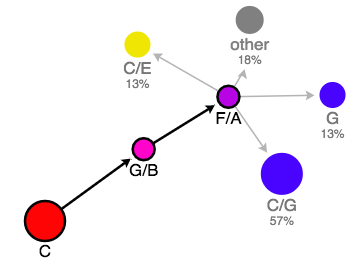
\includegraphics[width=.35\textwidth]{graphics/hook_theory_example.png}
  \caption{A graphical representation of a Markov model as learned and rendered by Hooktheory.com. In this representation, a context (of length 3) has been selected and the transition probabilities to the next chord are shown.}
    \label{fig:hook_theory}
\end{figure}

For this reason, we plan to train our own diversified model. Tab data, labeled by segment and with the inspiring emotion, would serve very well for this purpose. Songs would first be transposed to a single key. Assuming a Markov order of $m$ and $n$ possible chord labels (including alterations and added intervals), $n^m$ possible transitions exist. For even small values of $m$, this results in a large number of transitions (given that $n$ is in the thousands). In reality, a very small subset of the possible transitions are actually observed. If after looking at the power of the model we observe there are still too many transitions, there are effective ways to reduce $n$. In the limit, we can ignore everything but the root note (e.g., C) and the chord quality (i.e., major or minor), thereby limiting $n$ to 24. This practice is notably used in~\cite{steedman1984generative}.

One concern that might be raised relating to our use of tablature data is that the quality of transcriptions is often suboptimal. This is most commonly due to lack of expertise and not lack of attention to detail, which results in \emph{patterns} of errors in the data. We propose that such data is yet sufficient for our purposes as it still represents a human-generated creative artifact (though perhaps not that of the original composer). Consider, for example, that the tab used for the structure elucidation in Figure~\ref{fig:piano_man_chord_suffix_structure} contains a number of chords that we consider to have been incorrectly transcribed.

It is commonly noted that pop songs suffer from an over-repetition of certain chord progressions (e.g., I-IV-V). Although there are sound mathematical relationships which explain the stability of these chord sequences, it may be desirable to generate a wider variety of harmonies. One way to do this would be to equalize probabilities in the model according to some parameter, which in the limit would make all transitions (seen at least once in the data) of equal probability. Adjusting this parameter would then determine the amount of novelty and/or surprise in the harmonic progression.

Repetitions of chords in phrases or groups of phrases will be pre-determined by substructural elements. In this way we hope to approximate what Keller 2014 calls ``idiomatic chord progressions'' which are chord sequences that repeat in places throughout a composition.

%A chord progression (without melody) is not considered plagiarized, even if copied for an entire song. Even if permissible however, adding the non-plagiaristic constraint to harmony generation would be an interesting addition to the model in order to generate previously unseen harmonic progressions. Plagiarism in Markov sequence generation is considered in~\cite{papadopoulos2014avoiding}.

We will initially make the simplifying assumption of a single chord per measure and leave the consideration of multiple chords per measure (and their spacing) for future work.

\subsection{Melody}

Melody, like lyrics and harmony, is capable of (more or less) effectively conveying the inspiring idea. \emph{Melody} consists of a sequence of notes, each of which has a pitch (or rest) and a duration. The range of valid pitches corresponds to the MIDI note numbers, though in practice we will limit the range further to achieve melodies whose range is transposable into a singable range (e.g., 43-67). The minimum duration (which we will consider) corresponds to a 1/48 note to allow for triplet sixteenth notes as well as sixteenth notes. The maximum duration will be a whole note. The task of generating rhythms is commonly separated as precursory to generating pitches. It may be that they can or should be treated jointly, but for the sake of simplicity, we intend to follow this common practice.

%\begin{figure}
%  \centering
%  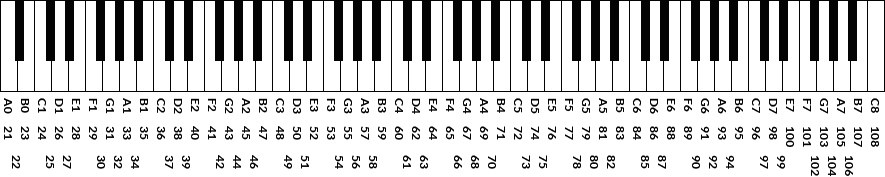
\includegraphics[width=\textwidth]{graphics/pitch-to-midi.png}
%  \caption{A standard 88-note keyboard labeled with the corresponding MIDI note numbers.}
%    \label{fig:pitch-to-midi}
%\end{figure}

\subsubsection{Rhythm}

The sequence of note (and rest) durations is what is defined as \emph{rhythm}. The particular rhythm of a melody determines in large measure which (corresponding) syllables receive emphasis. Rhythms that appropriately emphasize strong syllables contribute to a more natural pronunciation and comprehension of the lyrics. As an example, consider the line ``I'M a LIT-tle TEA-POT'' (traditionally sung in 4/4) in which each of the 4 beats of the measure coincide with a strong syllable in the lyrics (i.e., those capitalized). The pronunciation becomes more forced and the lyrics less comprehensible if, instead, we alter the rhythm to align the following capitalized syllables with beats 1-4: ``i'm A lit-TLE tea-POT war-MER''. Good rhythms avoid placing weak syllables on the principle beats of the measure.

A baseline solution to the problem of generating rhythm is to randomly select note durations within a more conservative range of durations (e.g., 1/8 to 1/2 notes). 

A more creative solution is  to sample durations from a distribution of rhythms learned from data. We might also consider sampling a multivariate distribution which in addition considers the position in the measure for which the duration is being sampled.

Another creative solution is modeled by~\cite{monteith2012automatic} who use a rhythm dictionary, learned from data, to generate new melodic rhythms. Their unique spin is to generate 100 rhythms in this way, use the CMU Pronunciation Dictionary to determine the stress patterns of the phonemes constituting the pre-generated lyrics, and then score each of the 100 rhythms based on how well the downbeats of each measure correspond with stressed syllables. In our estimation, this method might be improved upon by ensuring that, more than considering just the downbeat, as many stressed syllables as possible are aligned with beats. For this reason, we propose to use the stress patterns in the pre-generated lyrics to generate the rhythm, assigning durations according to a dynamic probabilistic model that gives highest probability to durations that would place the next strong syllable on the next beat.

\subsubsection{Pitch}

The generation of pitches to form interesting melodies has been the subject of significant research. A baseline solution to generating pitches simply chooses random pitches from those belonging to the triads of the accompanying chords. 

A more creative solution to generating pitch is to use a Markov chain to probabilistically choose the next pitch based on the contextual sequence of preceding pitches. The model would also be conditioned on the position in the measure for which the pitch is being determined and the current chord in the harmonic progression.

A second creative solution, rather than than generating pitch note by note, is to first define a sequence of idiomatic expressions similar to Keller's idiomatic chord progression bricks, Pachet's PACTs, or Murray's melody shapes~\cite {keller2013automating,pachet1991representing,murray2012algorithmically}. Each of these expressions essentially defines a contour or feature that the group of notes at a particular point in the sequence should form. For example, a rising line, a descending arpeggio, an oscillation between two neighboring notes, etc. This can also be accomplished using mathematical regression. 

The key signature of the composition will not be determined until after the melody has been generated. This is so that based on the melody, a key can be selected that maximizes singability within a determined vocal range.

Most effective compositions combine the melody and lyrics in a way that achieves an effect that is greater than the sum of parts. As an example, the contour or features in the melody can be made to accentuate the effect of the lyrics (this is called \emph{prosody}). Consider such well-known lines as ``\emph{stop} in the name of love,'' ``somewhere over the rainbow way \emph{up} high,'' and ``and I'm \emph{free}, free \emph{fallin'}.'' In these lines, the italicized words are emphasized by the melodic features that they suggest. This has been minimally studied in the context of CC and is an issue we feel deserves attention.

Here, as with lyrics, we would do well to address the issue of avoiding plagiarism, meaning the verbatim copying of melodies from instances in the training data whether intentionally or inadvertently through the generative process. Though significant work might be invested in this vein (cf.~\cite{papadopoulos1999ai}), it might be resolved by simply changing, adding, or deleting a few notes (either randomly or in accordance with a trained model) in order to create a novel melody.

\subsection{Voicing}

Having defined the lyrics, the harmony, and the melody, we have now generated a lyrical song in what is essentially defined as a \emph{leadsheet}. Voicing refers to how the song is then performed, including instrumentation, dynamics, tempo, and how the various harmonic voices will (or will not) be represented. The decision of which notes in the harmony will be voiced and how they will complement the melody is a critical element that has as much of an impact on the perception of the song as the composition itself~\cite{papadopoulos1999ai}.

This problem has been addressed in various places in the CC literature but is not of primary interest to our study. For our purposes, the composition itself is the creative artifact and its interpretation by performers is itself another. Countless artists have covered the popular Beatles song ``Yesterday,'' each applying his/her own creative voicing of the original creative masterpiece.

In order to allow those unfamiliar with reading leadsheets to evaluate our artifacts, we plan to implement a simple voicing module consisting of a male tenor voice singing the lyricized melody to a simple piano accompaniment which voices the harmony. Evaluation will be strictly limited to the non-voiced elements.

\subsection{Data}

We currently have access to a dataset of over 800,000 pop tabs. These tabs, in free-form, unstructured text, generally contain lyrics and chord sequences. With the help of other resources, additional metadata might be added to include information such as the author, specific genre, and key.

Only a small percentage of these tabs have global structure that is clearly labeled, raising the question, ``can global structure be inferred from just the chords and lyrics?'' Labeling the sections of a song is second-nature to humans when listening to an acoustic recording. However, when only considering the chords and lyrics, the task is ill-defined. Unlike in many other genres, in pop music there are no rules which prescribe compositional or segment lengths. In some rare cases, pop songs may depart almost entirely from having typical verse-chorus segments (e.g., Queen's ``Bohemian Rhapsody'' or the Beatles' ``You Never Give Me Your Money'').

One approach to elucidating global structure from an unlabeled tab is to perform (fuzzy) pattern matching of chord sequences within the song to find repeated segments (e.g., verses). To this end, we have experimented using a suffix tree (see Figure~\ref{fig:suffix_tree_piano_man}) that can be queried in constant time to find all instances of a chord subsequence of arbitrary length. Our preliminary results show promise, but we predict that observing patterns in the lyrics (e.g., choruses) will further improve results. 

\begin{figure}
  \centering
  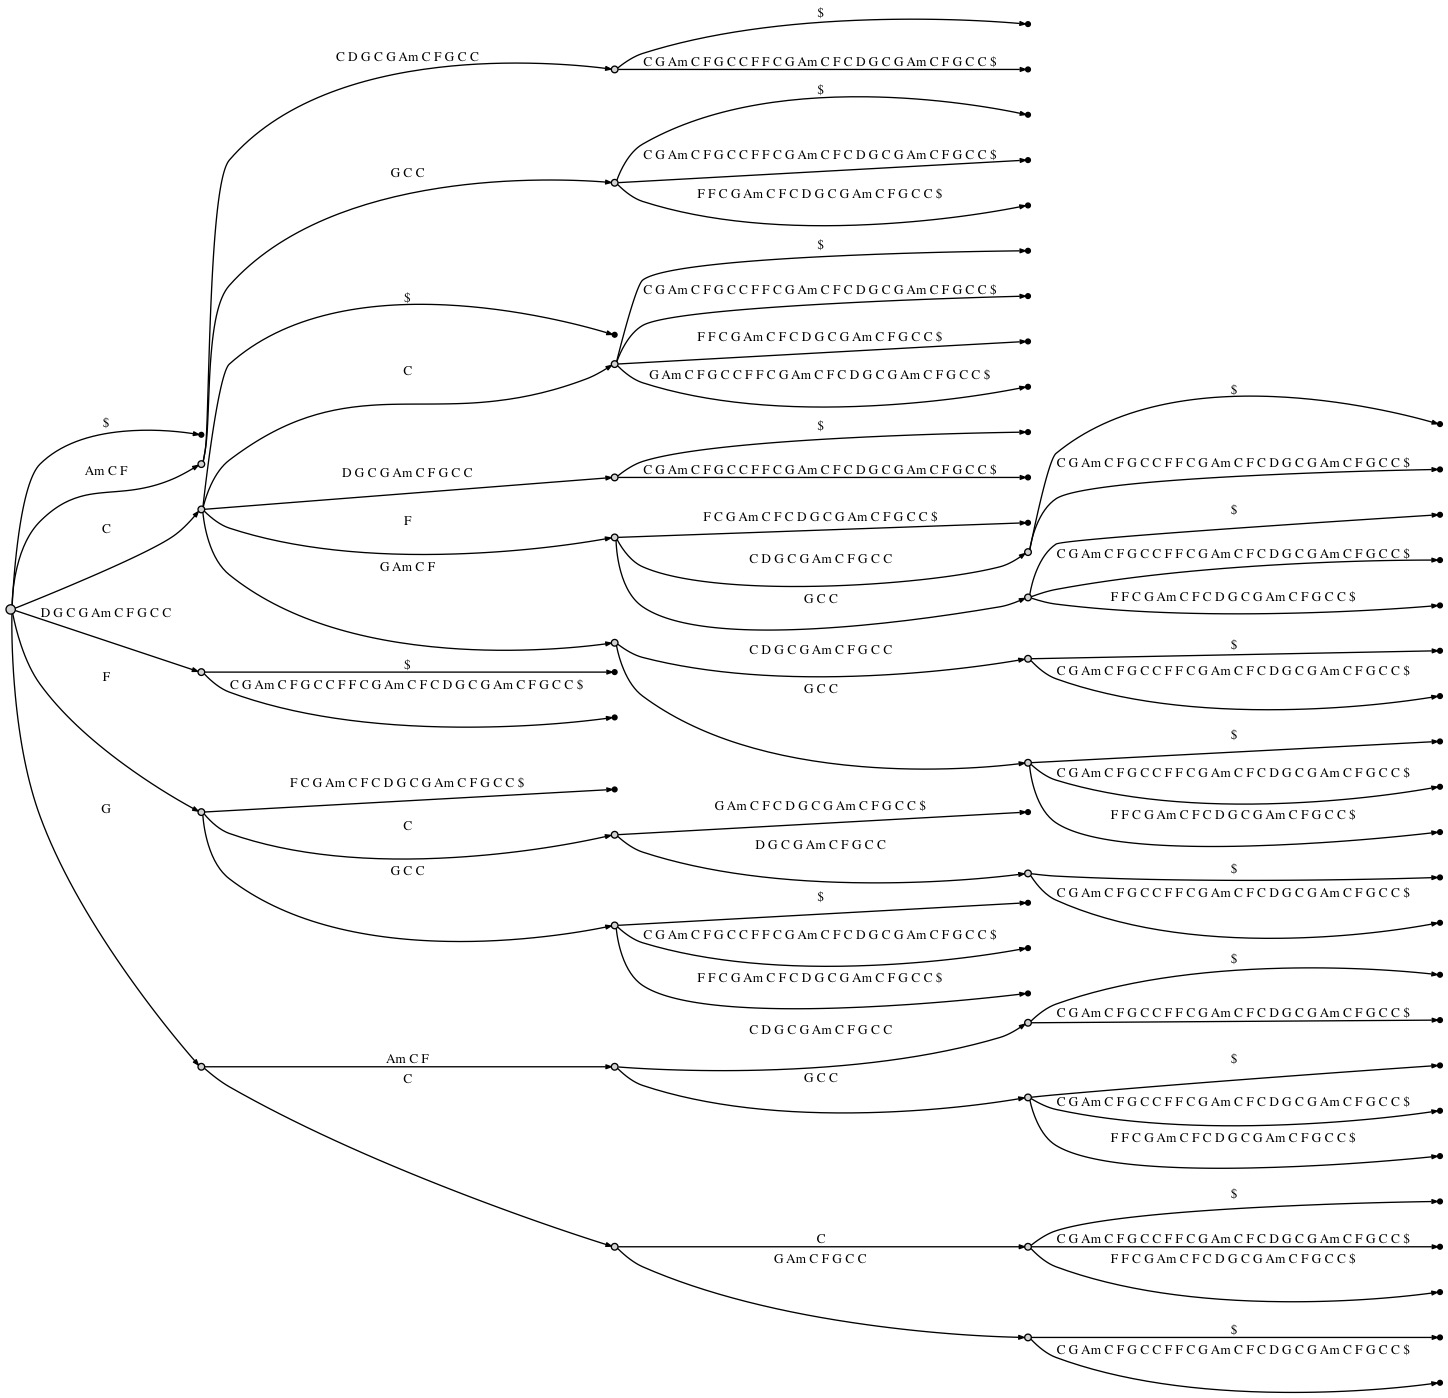
\includegraphics[width=.5\textwidth]{graphics/suffix_tree_piano_man.jpg}
  \caption{A graphical representation of the suffix tree created from the chord sequence of the first verse of ``Piano Man''. The suffix tree contains suffixes of the chord progression as keys and the suffix start positions as values. Such a suffix tree can be queried in constant time to find all instances of a chord subsequence of arbitrary length.}
    \label{fig:suffix_tree_piano_man}
\end{figure}

It may be unnecessary for a generative system to explicitly learn and model global verse-chorus structure if, by indirect means, it is capable of generating artifacts containing this structure. Using a suffix tree like that pictured in Figure~\ref{fig:suffix_tree_piano_man} but for all segments of ``Piano Man'', we incrementally identified the largest non-overlapping blocks of repeated subsequence until at least 90\% of the sequence was contained in blocks (existing blocks were subdivided as new blocks with common sequence were identified). The resulting segmentation of ``Piano Man'', as seen in Figure~\ref{fig:piano_man_chord_suffix_structure}, though unintuitive compared to a traditional verse-chorus structure, effectively captures a global structure of repetition (based solely on the chord sequence). This might suggest that global structure can be generated implicitly through hierarchical repetition of subsequences. We are interested in comparing this approach with the explicit modeling of global structure, suspecting that the latter will produce songs whose structure fits more easily into the range of expectation of most listeners.

\begin{figure}
  \centering
  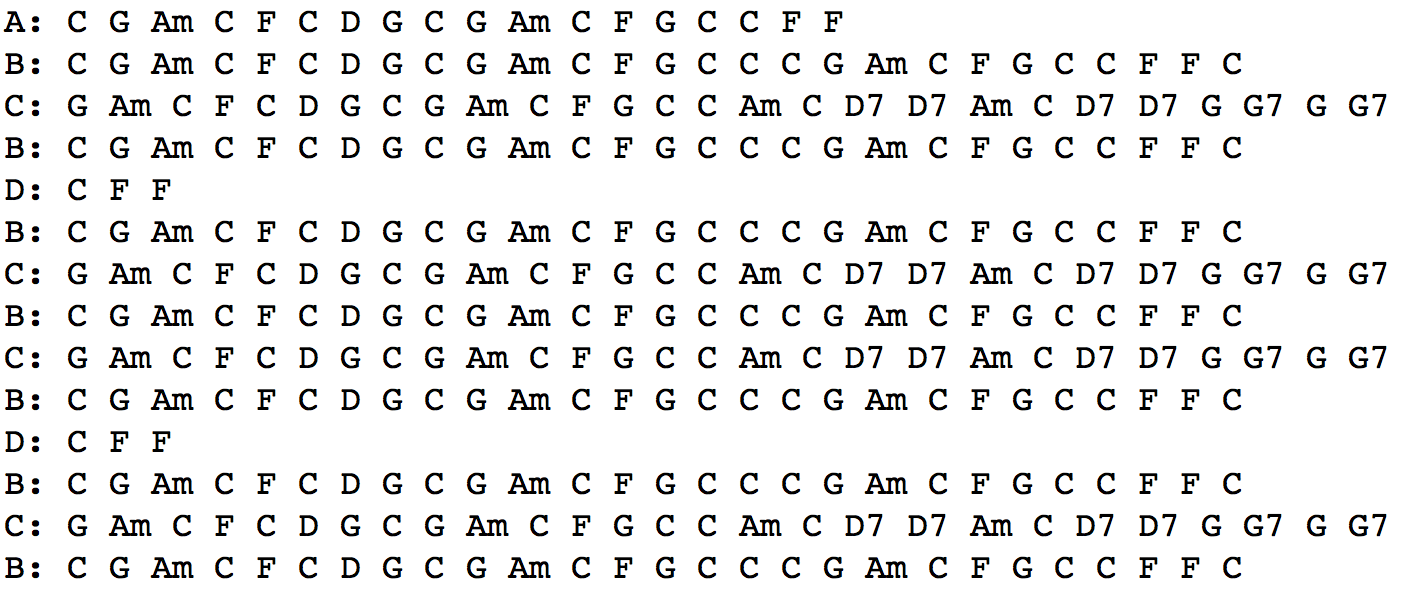
\includegraphics[width=.75\textwidth]{graphics/piano_man_chord_suffix_structure.png}
  \caption{Using a suffix tree like that in Figure~\ref{fig:suffix_tree_piano_man}, we algorithmically segmented the chord sequence of ``Piano Man'' based on repetitive subsequence. The blocks roughly represent the following segments: A---introduction; B---the first half of the verse or the entire chorus; C---the second half of the verse; D---the last of the chorus.}
    \label{fig:piano_man_chord_suffix_structure}
\end{figure}

Melody models cannot be trained from tablature data but will require an alternative data source, such as MIDI files. Several sites exist with freely available MIDI files for pop music.

%\subsection{Proof of concept}
%
%As a proof of concept, Figure x shows a composition created using this modular approach to pop song composition. In each case, we have used the simple solution proposed for each step for generation. Though certainly novel, it lacks surprise and value. Our goal will be to develop the more intelligent approaches described above in order to devise what might be deemed a more creative system.

%%%%%%%%%%%%%%%%%%%%%%%%%%%%%%%%%%%%%%%%%%%%%%%%%%%%%%%%%%%%%%%%%%%%%%%%%%%%%%%
\section{Validation}
% 1-2 pages
% Answers:
% 5) How can you demonstrate that this is a good solution?
%\subsection{Data}
%Tabs, dna, sheet music
%
%\subsection{Metrics}
%Combination of systemic evaluation and human evaulation.
%novel
%surprise
%value

%How will you demonstrate whether or not this is a good solution?

The question we set out to ask is, ``can we simulate creative behavior?''. Whereas AI generally describes well-defined problems with optimal outcomes against which AI solutions can be ranked and/or adapted, typically no ideal outcome exists for endeavors in CC. As per the definition of CC, the success of a CC system depends on exhibiting ``behaviors that unbiased observers would deem to be creative''. We need to ask people if they think that our artifacts are of sufficient quality to be enjoyable---to inspire the music's intended emotion. 

An important part of our research will be to develop effective qualitative surveys that allows us to convincingly demonstrate creativity. We will apply this metric to both novel generated pop songs as well as real (successful) pop songs. Our hope is that we will have at least a few songs that are received with as much success (via our questionnaire) as real pop songs written by professional musicians. We describe here the criteria that define creativity, followed by an example questionnaire designed to assess for these criteria. In addition to globally assessing for creativity, we plan to assess for creativity at each song-writing step, thus allowing incremental development of the sub-models of our computational composer. These modular assessments will use similar questionnaires to those designed to assess global creativity.

Despite lacking objective criteria upon which to define creativity, general qualities of creative behaviors have been repeatedly cited in CC literature. The two most common definitions are are those provided by Boden and Ritchie. Boden~\cite{boden2004creative} defines creativity in terms of novelty, surprise, and value. Ritchie~\cite{ritchie2007some} evaluates creativity using novelty, typicality, and quality. We will discuss how these notions relate and ultimately settle on Boden's definition for demonstrating creativity in our artifacts.

In words attributed to Igor Stravinsky, ``lesser artists borrow, great artists steal.'' \emph{Novelty} is generally assessed as a real-valued function, expressing a degree of similarity to pre-existing artifacts. In considering global structure, novelty can be assessed according to how many times (if any) a generated structure (in its entirety) has been previously used (as per available data). In this case we are less concerned about computing similarity between non-identical structures because structure is highly reused or largely similar between compositions (and can at times vary only as a matter of subjective opinion). With harmony, novelty can be determined as a product of the novelties of all chord subsequences. Using this function, novelty is computed for one or several fixed lengths (the length determining a specific granularity) and is also computed as an interpolation of several lengths (reflecting a more comprehensive novelty estimate). Novelty in lyrics and melody would be similarly evaluated.

Closely related to novelty is \emph{typicality}, the notion that an object fits within the definition of a particular artifact domain. Though highly formulaic, pop music does not generally adhere to specific rules about what does and does not constitute a pop song. There is extensive variation in the lengths, ranges, and complexities of global structure, lyrics, harmony, and melody. Any constraints we might impose in this regard to favor typicality are more likely to represent statements of what is \emph{valued} in a pop song (see below), not how it is defined. To this end, we will withhold from incorporating typicality measures in our modular fitness functions.

\emph{Surprise} refers to the unlikeliness or the interestingness of an artifact or behavior~\cite{boden2004creative}. A common approach to evaluating surprise is the use of information theory~\cite{meyer2008emotion}. In essence, when generating a musical sequence (e.g., any of the modular elements of composition), the \emph{expectation} can be computed for any of the possible successive symbols. Generations with high expectation are likely to be good artifacts but are in some sense less interesting. Controlled generation of less expected sequences is one way to introduce surprise to the listener. Surprise might thus be thought of as knowing the ``rules'' of the art and intelligently breaking them. We would like to have neither too much nor too little surprise. We will learn from data both the magnitude and patterns of surprise in successful popular music and use this range in our development of modular fitness functions.

\emph{Value}, as Boden notes, is the characteristic in which ``many arguments about creativity are rooted''~\cite{boden2004creative} (emphasis added). Defining value (or \emph{quality}, as ~\cite{ritchie2007some} calls it) is more difficult than defining previous attributes, in part because it is so subjective; what one listener enjoys, another may hate and vice versa. Several rules have been suggested for producing successful songs (e.g., ``get to the chorus within the first minute of the song'', ``only use a pre-chorus if the verse is short'', ``a bridge or instrumental solo should not come before the second chorus''), and as a first approach we will attempt to utilize these rules. But numerous, extremely successful counterexamples exist for each of these rules, encouraging the notion that we should explore breaking the rules.

We will demonstrate novelty, surprise, and value in our model using human questionnaires at each step of the modular development. For each module, we will control the other module variables by assigning them values taken from existing (less well-known) pop music (e.g., as done in~\cite{monteith2012automatic}). This way we can directly compare our generated artifacts for each component against A) other computationally creative systems which attempt to address the same tasks and B) other human-derived solutions. We will know our system has succeeded when, given no knowledge about the composition's composer, the creativity perceived in our generated artifacts is equivalent to or greater than that perceived in others (i.e., a Turing test). Questionnaires will involve questions (regarding cohesion, complexity, interestingness, novelty, etc.) about the overall composition as well as about the specific module being evaluated.

Often value is ascribed not only based on the artifact itself (cf.~\cite{ritchie2007some} for a counterargument) but also based on the process that brought it about~\cite{colton2012computational}. Norton et al. \cite{norton2015accounting} use a series of surveys in which the origin and creative process behind artifacts under comparison are A) masked, B) stated briefly, and C) given in detail. Their purpose is to consider the effects of responder bias given the different amounts of information. We propose conducting a similar series of surveys but with an added questionnaire which masks the origin (i.e., human vs computer) while still managing to disclose information about the creative process. A successful system will be perceived as being at least as creative with human composers when the details are masked. If the computer is viewed as at least as creative as humans even with details \emph{not masked}, then this would represent an even more convincing argument that the computer, based on the merits of its creations, is exhibiting creative behavior. This would allow improved separation of the potentially confounding effects of bias towards computer systems and bias resulting from knowledge of the creative process.

Lastly, we are interested in how well we communicate through music. To this end we would propose implementing a questionnaire which seeks to determine for each of several generated songs which emotion is perceived. The responses can then be compared to the inspiring emotions used to originally generate the songs (cf.~\cite{monteith2010automatic}). In a similar vein, we can tune fitness functions to create songs which demonstrate particular attributes (or lack thereof). We will know we have succeeded when information gathered via the questionnaires reflects that the applied filter achieves the desired perception. We are considering the possibility of staging a concert with live singers and a mix of human- and computer-generated music. Questionnaires would then take the form of an audience texting results during a live concert.

An example questionnaire might include: 
\begin{itemize}
\item{``On a scale of 1-5, how \emph{good} is this song?''}
\item{``On a scale of 1-5, how \emph{creative} is this song?''}
\item{``On a scale of 1-5, how well do you like the \emph{structure} of the song?''}
\item{``On a scale of 1-5, how much is this song like other pop songs you have heard?''}
\item{``On a scale of 1-5, how ``\emph{catchy}'' is this song?''}
\item{``On a scale of 1-5, how well do the chorus and the verse go together in this song?''}
\item{``Could you imagine hearing this song on the radio?''}
\item{``Would you like an MP3 recording of this song?'}
\item{``Would you pay \$1.00 for an MP3 recording of this song?'}
\item{``Which of the following emotions are evoked by listening to this song?''}
\item{``Which of the following songs was composed by a professional musician?''}
\item{``Please identify the chorus of this song.''}
\end{itemize}

%%%%%%%%%%%%%%%%%%%%%%%%%%%%%%%%%%%%%%%%%%%%%%%%%%%%%%%%%%%%%%%%%%%%%%%%%%%%%%%
\section{Thesis Schedule}
% about 1/2 page
% specifying dates for completion of major milestones, including potential
% papers and their submission dates
\begin{itemize}
\item{November 2016 - Get formatted tab data}
\item{February 27, 2016 - Papers submitted to the International Conference on Computational Creativity (ICCC) 2016:}
\begin{itemize}
\item{Summary of prospectus idea}
\item{``Structure elucidation and learning in western pop music''}
\item{``Computational creativity: to what end?''}
\end{itemize}
\item{April 2016 - Paper on ``Generating harmony in western pop music'' submitted to the Journal of New Music Research}
\item{September 2016 - Paper on ``Generating melody in western pop music'' submitted to the International Conference on Evolutionary and Biologically Inspired Music, Sound, Art and Design 2016 or Computer Music Journal}
\item{January 2017 - Papers submitted to ICCC 2017:}
\begin{itemize}
\item{``Generating lyrics in western pop music''}
\item{``Is all creativity computational?''}
\end{itemize}
\item{January 2017 - Submit dissertation to committee}
\item{February 2017 - Submit musical work to the 43rd International Computer Music Conference}
\item{March 2017 - Dissertation defense}
\item{April 2017 - Paper that puts it all together submitted to Digital Creativity, AI Magazine, or Minds and Machines}
\end{itemize}


%%%%%%%%%%%%%%%%%%%%%%%%%%%%%%%%%%%%%%%%%%%%%%%%%%%%%%%%%%%%%%%%%%%%%%%%%%%%%%%
% Change these to reflect the bibliography style and bibtex database file you want to use
\bibliographystyle{plain}
\bibliography{bib.bib}

\end{document}
